% ══════════════════════════════════════════════════════════════════════════
% Deep CFR, explained — a pedagogical companion for the PokerTrainer project
% Build:  pdflatex deep_cfr_tutorial.tex  (run twice for refs)
% ══════════════════════════════════════════════════════════════════════════
\documentclass[11pt,a4paper]{article}

\usepackage[utf8]{inputenc}
\usepackage[T1]{fontenc}
\usepackage{lmodern}
\usepackage[margin=2.2cm]{geometry}
\usepackage{amsmath,amssymb}
\usepackage[dvipsnames]{xcolor}
\usepackage{tikz}
\usetikzlibrary{arrows.meta,positioning,shapes.geometric,calc,fit,backgrounds}
\usepackage{listings}
\usepackage{tcolorbox}
\usepackage{booktabs}
\usepackage{enumitem}
\usepackage[colorlinks=true,linkcolor=MidnightBlue,urlcolor=MidnightBlue,citecolor=MidnightBlue]{hyperref}

% ─── Palette ────────────────────────────────────────────────────────────────
\definecolor{accent}{RGB}{25,55,110}     % deep blue
\definecolor{heroG}{RGB}{20,110,60}      % traverser green
\definecolor{villR}{RGB}{160,40,40}      % opponent red
\definecolor{memO}{RGB}{190,110,10}      % memory orange
\definecolor{codebg}{RGB}{246,247,249}
\definecolor{codekw}{RGB}{0,80,160}
\definecolor{codecomment}{RGB}{100,120,100}
\definecolor{codestr}{RGB}{150,60,20}

% ─── Code style ─────────────────────────────────────────────────────────────
\lstdefinestyle{py}{
  language=Python,
  basicstyle=\ttfamily\small,
  keywordstyle=\color{codekw}\bfseries,
  commentstyle=\color{codecomment}\itshape,
  stringstyle=\color{codestr},
  backgroundcolor=\color{codebg},
  frame=single, rulecolor=\color{black!25},
  framesep=6pt, xleftmargin=10pt, xrightmargin=4pt,
  showstringspaces=false,
  columns=fullflexible, keepspaces=true,
  breaklines=true,
  morekeywords={yield_from}
}

% ─── Pedagogical boxes ──────────────────────────────────────────────────────
\newtcolorbox{intuition}{
  colback=blue!4, colframe=accent, boxrule=0.8pt, arc=2mm,
  title=\textbf{Intuition}, fonttitle=\color{white},
  left=6pt, right=6pt, top=4pt, bottom=4pt}
\newtcolorbox{trap}{
  colback=red!4, colframe=villR, boxrule=0.8pt, arc=2mm,
  title=\textbf{Trap (learned the hard way in this project)}, fonttitle=\color{white},
  left=6pt, right=6pt, top=4pt, bottom=4pt}
\newtcolorbox{defbox}{
  colback=black!3, colframe=black!50, boxrule=0.6pt, arc=2mm,
  left=6pt, right=6pt, top=4pt, bottom=4pt}

\setlength{\parskip}{4pt}
\setlength{\parindent}{0pt}

\title{\bfseries Deep CFR, explained\\[2mm]
\large A pedagogical companion: from regret matching to a neural GTO poker player\\[1mm]
\normalsize (with the practical lessons of the PokerTrainer project)}
\author{PokerTrainer documentation}
\date{June 2026}

\begin{document}
\maketitle

\begin{abstract}
This document explains, from first principles, how one builds a near-GTO
(Game-Theory-Optimal) poker agent with \emph{Deep Counterfactual Regret
Minimization} (Deep CFR, Brown et al.\ 2019). It is written to be read
top-to-bottom by someone who knows Python and basic probability but has never
touched game theory. Every concept comes with a diagram or Python pseudo-code,
and the final sections summarize the modern landscape of poker AI
(DeepStack, Libratus, ReBeL, Player of Games, AlphaHoldem) and the concrete
engineering lessons learned while implementing Deep CFR in this repository.
\end{abstract}

\tableofcontents
\newpage

% ════════════════════════════════════════════════════════════════════════════
\section{The problem: playing well when you cannot see everything}
% ════════════════════════════════════════════════════════════════════════════

Chess and Go are \emph{perfect information} games: both players see the whole
board. Poker is different — you see your own cards but not your opponent's.
This single fact breaks the tools that work for chess (minimax search,
AlphaZero-style self-play on states), because in poker \textbf{a ``state'' is
not enough}: the best action depends on a \emph{probability distribution} over
what the opponent may hold, and that distribution depends on how both players
have been playing. Strategies must be \emph{randomized}: if you only raise
with aces, observant opponents fold and your aces earn nothing.

\begin{defbox}
\textbf{Information set (infoset).} All game states a player cannot tell apart.
In heads-up poker, an infoset is: \emph{my hole cards + the visible board + the
betting history so far}. The opponent's hidden cards vary across the states
inside one infoset, and a strategy must choose the \emph{same} action
distribution for the whole infoset --- you cannot condition on what you cannot see.
\end{defbox}

\begin{center}
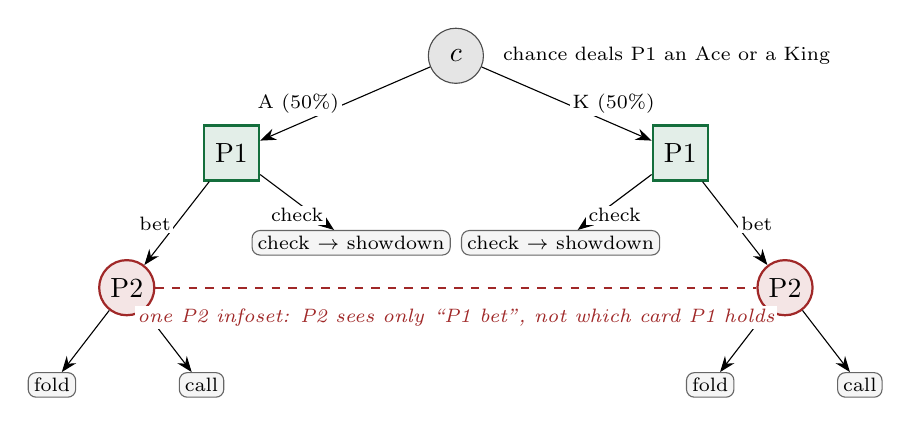
\begin{tikzpicture}[
  scale=0.95,
  cnode/.style={circle, draw=black!70, fill=black!10, minimum size=7mm, inner sep=1pt},
  p1/.style={rectangle, draw=heroG, fill=heroG!12, thick, minimum size=7mm, inner sep=2pt},
  p2/.style={circle, draw=villR, fill=villR!12, thick, minimum size=7mm, inner sep=1pt},
  term/.style={rectangle, rounded corners=1mm, draw=black!60, fill=black!4, inner sep=2pt, font=\scriptsize},
  edge label/.style={font=\scriptsize, fill=white, inner sep=1pt},
  >={Stealth[length=2mm]}]

  % chance root
  \node[cnode] (root) at (0,4.8) {$c$};
  \node[font=\scriptsize, anchor=west] at (0.5,4.8) {chance deals P1 an Ace or a King};

  % P1 nodes
  \node[p1] (p1a) at (-3.0,3.5) {P1};
  \node[p1] (p1k) at ( 3.0,3.5) {P1};
  \draw[->] (root) -- node[edge label, left=1pt]{A (50\%)} (p1a);
  \draw[->] (root) -- node[edge label, right=1pt]{K (50\%)} (p1k);

  % P1 actions: bet goes down-and-out to P2; check goes down-and-in to showdown
  \node[p2] (p2a) at (-4.4,1.7) {P2};
  \node[term] (ta)  at (-1.4,2.3) {check $\to$ showdown};
  \node[p2] (p2k) at ( 4.4,1.7) {P2};
  \node[term] (tk)  at ( 1.4,2.3) {check $\to$ showdown};
  \draw[->] (p1a) -- node[edge label, left=1pt]{bet} (p2a);
  \draw[->] (p1a) -- node[edge label, below=1pt]{check} (ta);
  \draw[->] (p1k) -- node[edge label, right=1pt]{bet} (p2k);
  \draw[->] (p1k) -- node[edge label, below=1pt]{check} (tk);

  % P2 terminals
  \node[term] (f1) at (-5.4,0.4) {fold};
  \node[term] (c1) at (-3.4,0.4) {call};
  \node[term] (f2) at ( 3.4,0.4) {fold};
  \node[term] (c2) at ( 5.4,0.4) {call};
  \draw[->] (p2a) -- (f1); \draw[->] (p2a) -- (c1);
  \draw[->] (p2k) -- (f2); \draw[->] (p2k) -- (c2);

  % the infoset: classic dashed link between the two indistinguishable nodes
  \draw[dashed, thick, villR] (p2a) -- (p2k);
  \node[font=\scriptsize\itshape, color=villR, fill=white, inner sep=1pt] at (0,1.30)
    {one P2 infoset: P2 sees only ``P1 bet'', not which card P1 holds};
\end{tikzpicture}
\end{center}

\begin{defbox}
\textbf{Nash equilibrium / GTO.} A pair of strategies such that neither player
can gain by deviating unilaterally. In two-player \emph{zero-sum} games (like
heads-up poker), playing a Nash strategy guarantees you cannot lose in
expectation, no matter what the opponent does. ``GTO play'' is the poker
community's name for it. The distance from equilibrium is called
\textbf{exploitability}: how much a perfect counter-strategy would win against
you. Solving a game $=$ driving exploitability toward $0$.
\end{defbox}

\begin{intuition}
GTO is \emph{defensive}: it does not try to exploit a weak opponent, it makes
\emph{you} unexploitable. That is exactly the right target for training:
it is a fixed mathematical object we can measure progress against ---
unlike ``beats opponent X'', which moves whenever X changes.
\end{intuition}

% ════════════════════════════════════════════════════════════════════════════
\section{Regret: the engine of everything}
% ════════════════════════════════════════════════════════════════════════════

Everything in CFR is built on one simple, almost embarrassing idea:
\emph{keep track of how much you regret not having played each action, and
play actions you regret in proportion to that regret.}

Let us make ``regret'' a number you could actually count. Fix \emph{one}
decision point, and suppose you have faced it 10 times so far, sometimes
folding, sometimes calling, sometimes raising. Adding up those 10 outcomes,
you won \textbf{5 chips in total}. Now replay history three times, each time
asking one question: \emph{what if I had played the same single action at
every one of those 10 visits, with everything else unchanged?}

\begin{center}
\small
\begin{tabular}{@{}lccc@{}}
\toprule
hindsight experiment & total chips & vs.\ the 5 you actually won & regret \\
\midrule
``I always fold''  & 3 & $3-5$ & $-2$ \\
``I always call''  & 8 & $8-5$ & $+3$ \\
``I always raise'' & 6 & $6-5$ & $+1$ \\
\bottomrule
\end{tabular}
\end{center}

The \textbf{regret of an action} is exactly that last column: what the action
\emph{would} have earned you, minus what you \emph{actually} earned. Positive
regret ($+3$ for \texttt{call}) means ``I wish I had played this more'';
negative regret ($-2$ for \texttt{fold}) means ``glad I didn't''. Collecting
the column into a vector, your cumulative regrets at this decision point are
$R = [-2, +3, +1]$. \textbf{Regret matching} (Hart \& Mas-Colell, 2000)
converts these into a strategy --- play each action in proportion to how much
you regret not playing it:

\begin{equation*}
\sigma(a) \;=\; \frac{\max(R(a),\,0)}{\sum_{b}\max(R(b),\,0)}
\qquad\text{(if all regrets} \le 0\text{: play } \arg\max_a R(a) \text{).}
\end{equation*}

\begin{center}
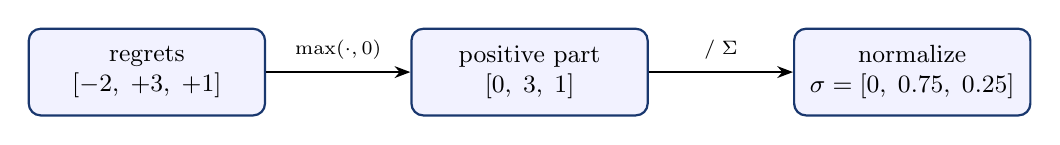
\begin{tikzpicture}[scale=0.9, font=\small, >={Stealth[length=2mm]},
  stage/.style={rectangle, rounded corners=1.5mm, draw=accent, fill=blue!5, thick,
                minimum height=11mm, minimum width=30mm, align=center}]
  \node[stage] (r)   at (0,0)    {regrets\\ $[-2,\;+3,\;+1]$};
  \node[stage] (pos) at (5.4,0)  {positive part\\ $[0,\;3,\;1]$};
  \node[stage] (sig) at (10.8,0) {normalize\\ $\sigma=[0,\;0.75,\;0.25]$};
  \draw[->, thick] (r) -- node[above=1pt,font=\scriptsize]{$\max(\cdot,0)$} (pos);
  \draw[->, thick] (pos) -- node[above=1pt,font=\scriptsize]{$/\;\Sigma$} (sig);
\end{tikzpicture}
\end{center}

\begin{lstlisting}[style=py, caption={Regret matching (the whole thing).}]
def regret_matching(R, legal):              # R: regret per action
    pos = [max(R[a], 0.0) for a in legal]
    z = sum(pos)
    if z > 0:
        return {a: p / z for a, p in zip(legal, pos)}
    # all regrets non-positive: play the least-bad action
    best = max(legal, key=lambda a: R[a])    # (ties: split equally)
    return {a: 1.0 if a == best else 0.0 for a in legal}
\end{lstlisting}

Why is this magic? Because of a classical theorem: if you keep updating regrets
and playing regret matching, your \emph{average} regret per round goes to zero
($O(1/\sqrt{T})$). And in two-player zero-sum games there is a beautiful
correspondence (the ``folk theorem'' of online learning):

\begin{defbox}
\textbf{If both players have average regret $\le \varepsilon$, the pair of
\emph{time-averaged} strategies is a $2\varepsilon$-Nash equilibrium.}
Self-play regret minimization $\Rightarrow$ convergence to GTO.
\end{defbox}

\begin{intuition}
Note carefully \emph{which} object converges: the \textbf{average} of all the
strategies you used across training, not the latest one. The current strategy
oscillates forever (it keeps probing); the \emph{average} of the oscillation is
the equilibrium. This is why Deep CFR ends with a separate ``average policy''
network --- it is the actual product of the whole procedure.
\end{intuition}

% ════════════════════════════════════════════════════════════════════════════
\section{CFR: regret, but at every infoset of a game tree}
% ════════════════════════════════════════════════════════════════════════════

Regret matching solves a single decision. A poker game is a \emph{tree} of
decisions. \textbf{Counterfactual Regret Minimization} (Zinkevich et al.\ 2007)
states that you can run an independent regret matcher \emph{at every infoset},
each fed with the right local quantity, and the global average strategy still
converges to Nash. The right local quantity is the \emph{counterfactual value}:

\begin{defbox}
\textbf{Counterfactual value} $v(I,a)$: the expected payoff of playing action
$a$ at infoset $I$, weighted by the probability that the \emph{others} (opponent
and chance) play into $I$ --- as if \emph{you} always tried to reach $I$.
The \textbf{instantaneous regret} of $a$ at $I$ under the current strategy
$\sigma_t$ is
$r_t(I,a) = v(I,a) - \sum_{b}\sigma_t(I,b)\,v(I,b)$,
i.e.\ ``action $a$ versus what I currently do on average at $I$''.
\end{defbox}

Vanilla CFR then loops: traverse the \emph{whole} tree, accumulate
$R_T(I,a)=\sum_t r_t(I,a)$ at every infoset, update every $\sigma$ by regret
matching, repeat. Here it is in full --- the bookkeeping to watch is the two
\emph{reach probabilities} carried down the tree, because each one is used for
a different purpose at the update:

\begin{lstlisting}[style=py, caption={Tabular vanilla CFR (two players, chance sampled once per traversal). The asymmetry to internalize: regrets are weighted by the \emph{opponent's} reach (that is what makes values ``counterfactual''), while the average strategy is weighted by \emph{your own} reach (you only average a decision where you would actually arrive).}]
R = defaultdict(zeros)     # cumulative regrets,  one vector per infoset
S = defaultdict(zeros)     # cumulative strategy, one vector per infoset

def cfr(state, t, reach):
    """reach[p] = probability that player p's OWN choices so far would
    lead them here. Returns (u_0, u_1), expected values under sigma_t."""
    if state.is_terminal():
        return state.payoffs()                  # zero-sum pair

    I, p  = infoset(state), state.to_act()
    sigma = regret_matching(R[I], state.legal())

    v, v_I = {}, [0.0, 0.0]
    for a in state.legal():
        r = list(reach)
        r[p] *= sigma[a]                        # my move scales MY reach
        v[a] = cfr(state.child(a), t, r)
        v_I[0] += sigma[a] * v[a][0]
        v_I[1] += sigma[a] * v[a][1]

    for a in state.legal():                     # ── the two updates ──
        R[I][a] += reach[1 - p] * (v[a][p] - v_I[p])   # OPPONENT's reach
    S[I] += reach[p] * sigma                           # MY OWN reach
    return v_I

def solve(T):
    for t in range(1, T + 1):
        cfr(deal_random_hand(), t, reach=[1.0, 1.0])   # chance sampled
    return {I: S[I] / S[I].sum() for I in S}    # AVERAGE strategy ~ Nash
\end{lstlisting}

Two practical refinements matter for us --- and both are tiny edits to the
update lines above:

\begin{itemize}[leftmargin=1.4em, itemsep=1pt]
\item \textbf{Linear CFR} (Brown \& Sandholm 2019): weight iteration $t$'s
      contributions by $t$. Early iterations are garbage (the strategy was
      random); weighting by $t$ discounts them and speeds convergence a lot.
\item \textbf{CFR$^{+}$} (Tammelin 2014): clip cumulative regrets at zero
      after every update, so an action can recover quickly once it stops
      being bad. (Used by the commercial GTO solvers and by Cepheus to
      essentially solve limit hold'em; Deep CFR uses Linear CFR instead.)
\end{itemize}

\begin{lstlisting}[style=py, caption={CFR$^{+}$ and Linear CFR are three-line edits to the two update lines.}]
# ── vanilla CFR ──────────────────────────────────────────────────────
R[I][a] += reach[1 - p] * (v[a][p] - v_I[p])
S[I]    += reach[p] * sigma

# ── CFR+ : clip cumulative regret at 0; average weighted by t ───────
R[I][a]  = max(R[I][a] + reach[1 - p] * (v[a][p] - v_I[p]), 0.0)
S[I]    += t * reach[p] * sigma
# (CFR+ also alternates: update one player's regrets per traversal)

# ── Linear CFR : weight EVERYTHING by the iteration number t ────────
R[I][a] += t * reach[1 - p] * (v[a][p] - v_I[p])
S[I]    += t * reach[p] * sigma
# equivalent in Deep CFR: store plain samples tagged with t, and weight
# the regression loss by t  (exactly what trainer/cfr/train.py does)
\end{lstlisting}

\begin{trap}
CFR's guarantee is about the \emph{average} strategy. Looking at the
\emph{current} network/strategy mid-training and judging ``it plays weird'' is
not, by itself, evidence of failure --- but a current strategy frozen at
uniform, or one that never discriminates hand strength, \emph{is} (see
Section~\ref{sec:lessons}).
\end{trap}

% ════════════════════════════════════════════════════════════════════════════
\section{Monte Carlo CFR: sample the tree instead of visiting it all}
% ════════════════════════════════════════════════════════════════════════════

Heads-up no-limit hold'em has about $10^{160}$ states. Vanilla CFR visits the
whole tree per iteration --- impossible. \textbf{External-sampling MCCFR}
(Lanctot et al.\ 2009) fixes this with one elegant asymmetry per traversal.
One player is the \emph{traverser} (we are computing \emph{their} regrets this
traversal):

\begin{center}
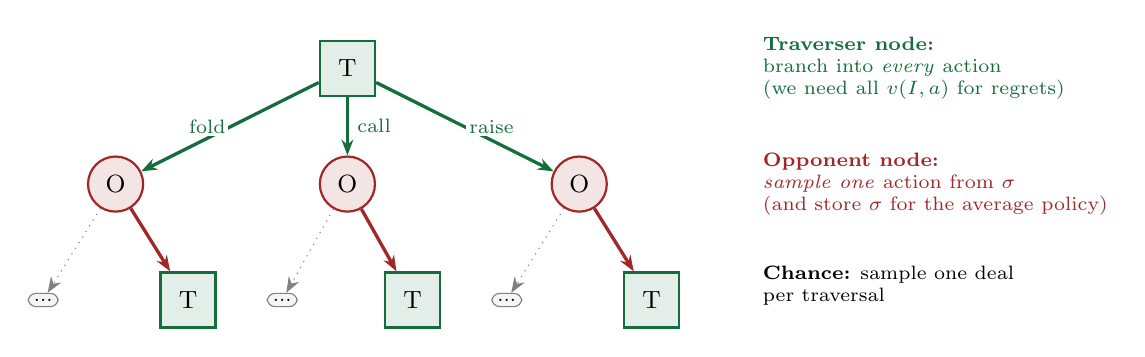
\begin{tikzpicture}[
  scale=0.92, font=\small, >={Stealth[length=2mm]},
  trav/.style={rectangle, draw=heroG, fill=heroG!12, thick, minimum size=7mm},
  opp/.style={circle, draw=villR, fill=villR!12, thick, minimum size=7mm, inner sep=1pt},
  term/.style={rectangle, rounded corners=1mm, draw=black!50, fill=black!4,
               inner sep=2pt, font=\scriptsize},
  lbl/.style={font=\scriptsize, fill=white, inner sep=1pt}]

  \node[trav] (t) at (0,4.2) {T};
  \node[opp] (o1) at (-3.2,2.6) {O};
  \node[opp] (o2) at (0,2.6) {O};
  \node[opp] (o3) at (3.2,2.6) {O};
  \draw[->, very thick, heroG] (t) -- node[lbl,left]{fold} (o1);
  \draw[->, very thick, heroG] (t) -- node[lbl,right=2pt]{call} (o2);
  \draw[->, very thick, heroG] (t) -- node[lbl,right]{raise} (o3);

  \node[term] (x1) at (-4.2,1.0) {...};
  \node[trav] (t2) at (-2.2,1.0) {T};
  \node[term] (x2) at (-0.9,1.0) {...};
  \node[trav] (t3) at (0.9,1.0) {T};
  \node[term] (x3) at (2.2,1.0) {...};
  \node[trav] (t4) at (4.2,1.0) {T};

  % opponent samples ONE action: solid; others dotted
  \draw[->, very thick, villR] (o1) -- (t2);
  \draw[->, dotted, black!50] (o1) -- (x1);
  \draw[->, very thick, villR] (o2) -- (t3);
  \draw[->, dotted, black!50] (o2) -- (x2);
  \draw[->, very thick, villR] (o3) -- (t4);
  \draw[->, dotted, black!50] (o3) -- (x3);

  \node[align=left, font=\scriptsize, anchor=west] at (5.6,4.2)
    {\textcolor{heroG}{\textbf{Traverser node:}}\\
     \textcolor{heroG}{branch into \emph{every} action}\\
     \textcolor{heroG}{(we need all $v(I,a)$ for regrets)}};
  \node[align=left, font=\scriptsize, anchor=west] at (5.6,2.6)
    {\textcolor{villR}{\textbf{Opponent node:}}\\
     \textcolor{villR}{\emph{sample one} action from $\sigma$}\\
     \textcolor{villR}{(and store $\sigma$ for the average policy)}};
  \node[align=left, font=\scriptsize, anchor=west] at (5.6,1.2)
    {\textbf{Chance:} sample one deal\\ per traversal};
\end{tikzpicture}
\end{center}

This sampling scheme has two crucial properties, both provable:
(1) the sampled regret estimates are \emph{unbiased}; and
(2) opponent infosets are visited with probability proportional to the
opponent's \emph{own} probability of reaching them under $\sigma$ ---
which is exactly the weighting needed when collecting strategy samples for
the average policy (more on this in Section~\ref{sec:deepcfr}, it caused a
real bug in this repo).

% ════════════════════════════════════════════════════════════════════════════
\section{Deep CFR: replace the tables with networks}\label{sec:deepcfr}
% ════════════════════════════════════════════════════════════════════════════

Even MCCFR keeps a \emph{table} of regrets, one row per infoset --- still
impossibly many in no-limit poker. Historically this was handled with
hand-crafted \emph{abstraction} (bucketing similar hands together).
\textbf{Deep CFR} (Brown, Lerer, Gross, Sandholm 2019) removes the tables and
the abstraction: a neural network \emph{generalizes} regrets across infosets.

\subsection{The three memories and two kinds of networks}

\begin{center}
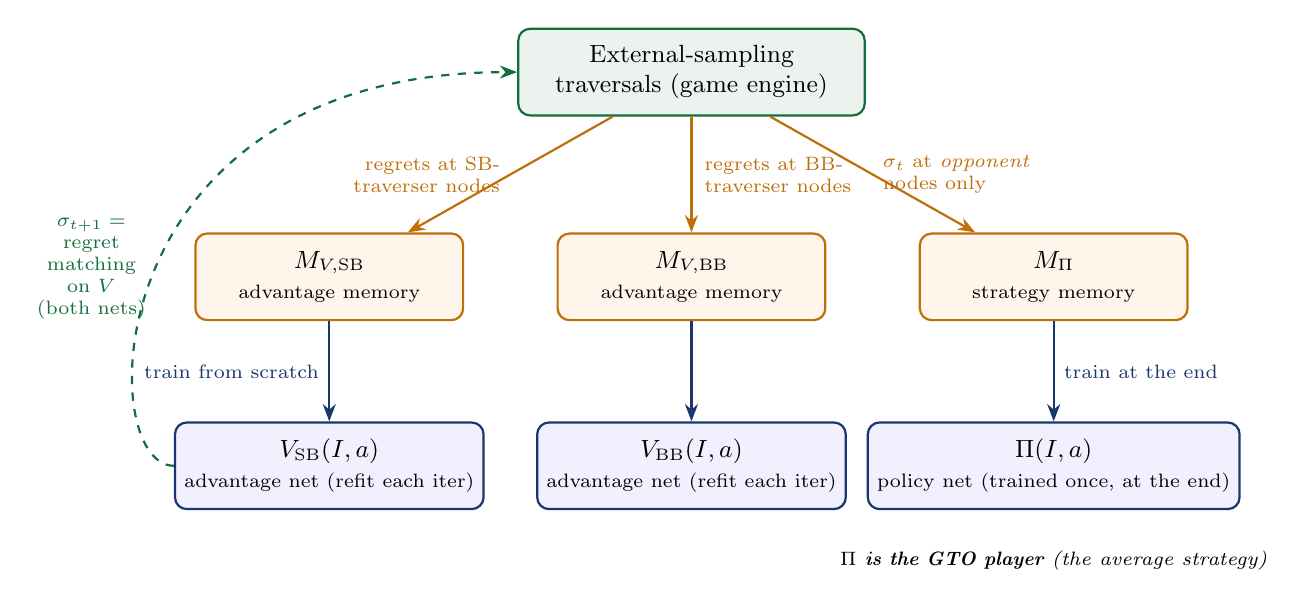
\begin{tikzpicture}[
  font=\small, >={Stealth[length=2.2mm]}, node distance=8mm,
  box/.style={rectangle, rounded corners=1.5mm, thick, align=center,
              minimum height=11mm, minimum width=34mm},
  netbox/.style={box, draw=accent, fill=blue!6},
  membox/.style={box, draw=memO, fill=orange!8},
  gamebox/.style={box, draw=heroG, fill=heroG!8}]

  \node[gamebox, minimum width=44mm] (trav) at (0,0)
    {External-sampling\\ traversals (game engine)};

  \node[membox] (mv0) at (-4.6,-2.6) {$M_{V,\mathrm{SB}}$\\ \scriptsize advantage memory};
  \node[membox] (mv1) at (0,-2.6)    {$M_{V,\mathrm{BB}}$\\ \scriptsize advantage memory};
  \node[membox] (mpi) at (4.6,-2.6)  {$M_{\Pi}$\\ \scriptsize strategy memory};

  \node[netbox] (v0) at (-4.6,-5.0) {$V_{\mathrm{SB}}(I,a)$\\ \scriptsize advantage net (refit each iter)};
  \node[netbox] (v1) at (0,-5.0)    {$V_{\mathrm{BB}}(I,a)$\\ \scriptsize advantage net (refit each iter)};
  \node[netbox] (pi) at (4.6,-5.0)  {$\Pi(I,a)$\\ \scriptsize policy net (trained once, at the end)};

  \draw[->, thick, memO] (trav) -- node[left, font=\scriptsize, align=right]
      {regrets at SB-\\traverser nodes} (mv0);
  \draw[->, thick, memO] (trav) -- node[right=1pt, font=\scriptsize, align=left]
      {regrets at BB-\\traverser nodes} (mv1);
  \draw[->, thick, memO] (trav) -- node[right, font=\scriptsize, align=left]
      {$\sigma_t$ at \emph{opponent}\\ nodes only} (mpi);

  \draw[->, thick, accent] (mv0) -- node[left, font=\scriptsize]{train from scratch} (v0);
  \draw[->, thick, accent] (mv1) -- (v1);
  \draw[->, thick, accent] (mpi) -- node[right, font=\scriptsize]{train at the end} (pi);

  % feedback loop: nets drive sigma in the next traversals
  \draw[->, thick, dashed, heroG] (v0.west) .. controls (-7.6,-5.0) and (-7.6,0) ..
      node[left, font=\scriptsize, align=center]{$\sigma_{t+1}=$\\ regret\\ matching\\ on $V$\\ (both nets)} (trav.west);

  \node[font=\scriptsize\itshape] at (4.6,-6.2) {$\Pi$ \textbf{is the GTO player} (the average strategy)};
\end{tikzpicture}
\end{center}

\begin{itemize}[leftmargin=1.4em, itemsep=2pt]
\item \textbf{Advantage networks} $V_p(I,a)$, one per player: trained to predict
  the (linearly weighted, time-averaged) regret of each action at infoset $I$.
  The current strategy is obtained by \emph{regret matching on the network's
  outputs}: $\sigma_t(I)=\mathrm{RM}(V_p(I,\cdot))$.
\item \textbf{Advantage memories} $M_{V,p}$: reservoir buffers of
  $(I,\,t,\,\tilde r_t(I,\cdot))$ samples collected at the traverser's nodes.
\item \textbf{Strategy memory} $M_\Pi$: reservoir buffer of $(I,\,t,\,\sigma_t(I))$
  samples collected at \emph{opponent} nodes only.
\item \textbf{Policy network} $\Pi$: trained \emph{once at the very end} on
  $M_\Pi$ --- it distills the time-averaged strategy, the thing that actually
  converges to Nash.
\end{itemize}

\subsection{The algorithm, in Python pseudo-code}

This is Algorithm~1 of the paper, written the way this repository implements it
(\texttt{trainer/cfr/cfr\_coro.py}):

\begin{lstlisting}[style=py, caption={One external-sampling traversal (the heart of Deep CFR).}]
def traverse(state, p, t):
    """Recursive traversal; returns the expected value for traverser p."""
    if state.is_terminal():
        return state.payoff(p)

    I     = infoset(state)                 # what the actor can see
    actor = state.to_act()
    legal = state.legal_actions()

    # current strategy at I = regret matching on the actor's advantage net
    sigma = regret_matching(V[actor](I), legal)

    if actor == p:                         # ── TRAVERSER node ──────────
        v = {}
        for a in legal:                    # branch into EVERY action
            v[a] = traverse(state.child(a), p, t)
        v_I = sum(sigma[a] * v[a] for a in legal)
        regrets = {a: v[a] - v_I for a in legal}
        M_V[p].reservoir_add((I, t, regrets))
        return v_I
    else:                                  # ── OPPONENT node ───────────
        M_Pi.reservoir_add((I, t, sigma))  # strategy sample (HERE only!)
        a = sample(sigma)                  # play ONE action
        return traverse(state.child(a), p, t)
\end{lstlisting}

\begin{lstlisting}[style=py, caption={The outer loop. Note the two unusual moves: networks are retrained \emph{from scratch} each iteration, and the deliverable is the policy net trained at the end.}]
def deep_cfr(T, K):
    for t in range(1, T + 1):
        for p in PLAYERS:                       # SB, BB
            for k in range(K):                  # K traversals per player
                state = deal_random_hand()      # chance is sampled
                traverse(state, p, t)
            V[p] = AdvantageNet()               # fresh net (from scratch!)
            fit(V[p], M_V[p],                   # regression on the memory
                loss=lambda pred, r, t_i: t_i * mse(pred, r))  # Linear CFR
    Pi = PolicyNet()
    fit(Pi, M_Pi, loss=lambda pred, sig, t_i: t_i * ce(pred, sig))
    return Pi                                   # the (near-)GTO player
\end{lstlisting}

\begin{lstlisting}[style=py, caption={Reservoir sampling (Vitter's Algorithm R): a fixed-size buffer that remains a \emph{uniform} sample of everything ever inserted --- this is what lets a finite memory represent all $T$ iterations fairly.}]
def reservoir_add(buf, item):
    buf.n_seen += 1
    if len(buf) < buf.capacity:
        buf.append(item)
    else:
        j = randint(0, buf.n_seen - 1)          # uniform over the stream
        if j < buf.capacity:
            buf[j] = item                       # replace a random slot
\end{lstlisting}

\subsection{Why each piece is the way it is}

\begin{intuition}
\textbf{Why predict regrets and not ``the best action''?} Because CFR's
convergence machinery runs on regrets. The network is just a compressed,
generalizing regret table: two infosets with similar cards and similar
histories share statistical strength instead of each needing its own row.
\end{intuition}

\begin{intuition}
\textbf{Why retrain from scratch each iteration?} The target ---
the time-averaged regret --- changes every iteration. Warm-starting from
the previous net biases the regression toward stale targets; the paper found
from-scratch refits more reliable. (It costs wall-clock time, which is why
the refit budget is a key hyperparameter.)
\end{intuition}

\begin{intuition}
\textbf{Why store strategy samples only at opponent nodes?}
External sampling makes the opponent play through its own nodes with
probability equal to its own reach --- so the stream of opponent-node
$\sigma$ samples is \emph{automatically} reach-weighted, which is the exact
weighting the average strategy needs. Traverser nodes are reached by brute
branching (every action, regardless of $\sigma$), so including them would
inject reach-\emph{unweighted} samples and bias the final policy.
\end{intuition}

\begin{trap}
This repository initially stored $\sigma$ at \emph{every} node ``to collect
more data''. More data, wrong distribution: the PolicyNet --- the actual output
of the algorithm --- was being trained on a biased average. Paper fidelity
matters most precisely where it is least obvious.
\end{trap}

\subsection{Small but load-bearing details}

\begin{itemize}[leftmargin=1.4em, itemsep=2pt]
\item \textbf{All-non-positive regrets $\Rightarrow$ argmax.} When
  $\sum_a \max(V(I,a),0)=0$, the paper plays the highest-advantage action
  \emph{deterministically}. Uniform would keep wasting opponent samples on
  known-bad actions.
\item \textbf{Iteration 1 must be uniform.} A freshly initialized network
  outputs noise; regret matching on noise gives a degenerate one-hot strategy
  that can collapse one player's traversal trees. Fix used here: zero-initialize
  the advantage net's output head, and make the argmax fallback split exact
  ties equally --- all-zero outputs then tie everywhere and degrade gracefully
  to uniform, with no special case in the traversal.
\item \textbf{Linear weighting lives in the loss.} Each sample carries its
  iteration $t$; the regression weights samples by $t$. This implements Linear
  CFR without ever touching stored targets.
\end{itemize}

% ════════════════════════════════════════════════════════════════════════════
\section{The modern landscape: ways to build a GTO player}
% ════════════════════════════════════════════════════════════════════════════

\begin{center}
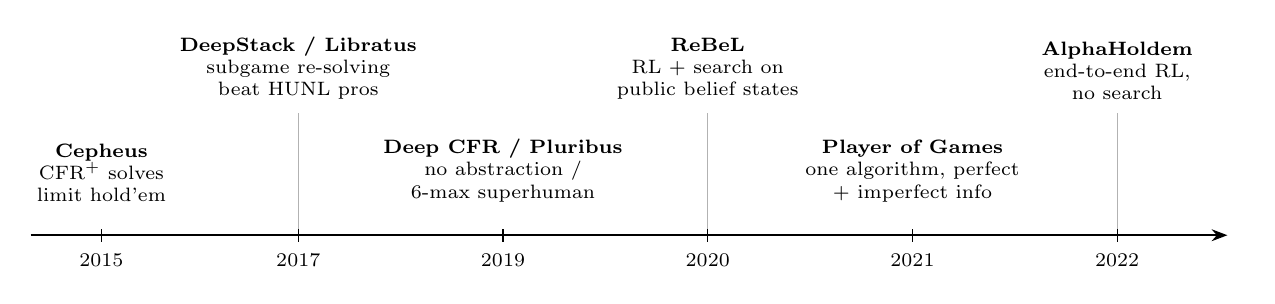
\begin{tikzpicture}[font=\scriptsize, >={Stealth[length=2mm]}]
  \draw[->, thick] (0,0) -- (15.2,0) node[right]{};
  \foreach \x/\y in {0.9/2015, 3.4/2017, 6.0/2019, 8.6/2020, 11.2/2021, 13.8/2022}
    \draw (\x,-0.08) -- (\x,0.08) node[below=2mm]{\y};
  % staggered labels: odd milestones low, even milestones high (guide lines up)
  \foreach \x in {3.4, 8.6, 13.8}
    \draw[black!30] (\x,0.08) -- (\x,1.55);
  \node[align=center, anchor=south] at (0.9,0.30)
    {\textbf{Cepheus}\\ CFR$^{+}$ solves\\ limit hold'em};
  \node[align=center, anchor=south] at (3.4,1.60)
    {\textbf{DeepStack / Libratus}\\ subgame re-solving\\ beat HUNL pros};
  \node[align=center, anchor=south] at (6.0,0.30)
    {\textbf{Deep CFR / Pluribus}\\ no abstraction /\\ 6-max superhuman};
  \node[align=center, anchor=south] at (8.6,1.60)
    {\textbf{ReBeL}\\ RL + search on\\ public belief states};
  \node[align=center, anchor=south] at (11.2,0.30)
    {\textbf{Player of Games}\\ one algorithm, perfect\\ + imperfect info};
  \node[align=center, anchor=south] at (13.8,1.60)
    {\textbf{AlphaHoldem}\\ end-to-end RL,\\ no search};
\end{tikzpicture}
\end{center}

Three families of approaches, with different trade-offs:

\textbf{1. Tabular CFR on an abstraction + subgame re-solving (2015--2017).}
Bucket strategically similar hands, solve the smaller game with CFR$^{+}$/MCCFR
(the ``blueprint''), then at play time re-solve the current subgame more finely
(\emph{Libratus}: nested safe subgame solving; \emph{DeepStack}: continual
re-solving with learned counterfactual-value networks as depth limits).
Strong but engineering-heavy; the abstraction is hand-crafted.

\textbf{2. Neural CFR without search (Deep CFR, 2019; this project).} Let a
network generalize across infosets; no abstraction, no play-time search ---
the policy net plays directly. Conceptually clean, single training loop;
the price is regression noise on regrets, so per-game exploitability is higher
than search-based systems. \emph{Pluribus} (6-max superhuman, 2019) is the
hybrid cousin: an MCCFR blueprint plus depth-limited re-solving at play time.

\textbf{3. RL + search on belief states (2020--).} \emph{ReBeL} casts the
imperfect-information game as a continuous-state perfect-information game over
\emph{public belief states} (distributions over private cards), and trains
value/policy nets by self-play with CFR used inside the search.
\emph{Player of Games} unifies this with AlphaZero-style search so one
algorithm plays chess, Go \emph{and} poker. At the other extreme,
\emph{AlphaHoldem} drops search entirely (pure actor-critic end-to-end) and
is much cheaper at play time, at some cost in robustness guarantees.

\begin{center}
\small
\begin{tabular}{@{}llllc@{}}
\toprule
System & Year & Core idea & Search at play time? & Nets \\
\midrule
Cepheus        & 2015 & CFR$^{+}$, essentially solved limit HU      & no  & --- \\
DeepStack      & 2017 & continual re-solving + CFV nets             & yes & value \\
Libratus       & 2017 & abstraction blueprint + safe re-solving     & yes & --- \\
Deep CFR       & 2019 & networks replace regret tables              & no  & value+policy \\
Pluribus       & 2019 & blueprint + depth-limited search (6-max)    & yes & --- \\
ReBeL          & 2020 & RL+search on public belief states           & yes & value+policy \\
Player of Games& 2021 & sound search for both info regimes          & yes & value+policy \\
AlphaHoldem    & 2022 & end-to-end actor-critic, no search          & no  & policy \\
\bottomrule
\end{tabular}
\end{center}

\begin{intuition}
The recurring trade-off is \textbf{search at play time}. Search buys lower
exploitability per unit of training but costs latency, complexity, and (in
belief-state methods) a tractable public state. Search-free methods (Deep CFR,
AlphaHoldem) give you a single network you can ship anywhere --- which is why
this project chose Deep CFR as its backbone.
\end{intuition}

% ════════════════════════════════════════════════════════════════════════════
\section{This project: Deep CFR with a token transformer and a curriculum}
\label{sec:project}
% ════════════════════════════════════════════════════════════════════════════

\subsection{Encoding the infoset as a token sequence}

Early versions encoded the infoset as one flat 816-dimensional vector; the
hole cards were 52 of those dimensions and the trained network simply
\emph{ignored them} (measured: the strategy varied by $<2\%$ across all 38
test hands). The fix was structural, not capacity: encode the infoset as a
\textbf{sequence of tokens} --- each card, action, pot-size bucket and
stack-size bucket gets its own token --- and use a small transformer.
Attention must then handle each card as a first-class object that cannot be
averaged away into 700 other dimensions.

\begin{center}
\ttfamily\small
[BOS] [POS\_SB] [Ah] [As] [SEP\_PRE] [HERO][R100][POT\_2][STACK\_15] \\
\hphantom{[BOS] }[VILLAIN][AI][POT\_9][STACK\_0] [DECISION]
\end{center}

The network reads the hidden state at the final \texttt{[DECISION]} token and
outputs one number per action (predicted regrets for the advantage net,
logits for the policy net). The same architecture serves both nets.

\subsection{Curriculum: solve an easy poker first}

Training the full 100bb game directly kept producing hand-agnostic strategies
(a chicken-and-egg: a hole-blind strategy generates hole-blind regret targets,
so the net correctly learns a constant function and nothing improves).
The project's answer is a \textbf{curriculum over the game itself}, keeping the
network's shape fixed across stages so weights transfer with a plain
\texttt{load\_state\_dict}:

\begin{center}
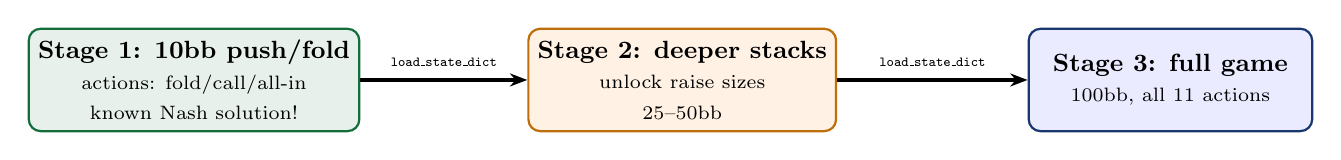
\begin{tikzpicture}[font=\small, >={Stealth[length=2.2mm]},
  st/.style={rectangle, rounded corners=1.5mm, thick, align=center,
             minimum height=13mm, minimum width=36mm}]
  \node[st, draw=heroG, fill=heroG!10] (s1) at (0,0)
    {\textbf{Stage 1: 10bb push/fold}\\ \scriptsize actions: fold/call/all-in\\
     \scriptsize known Nash solution!};
  \node[st, draw=memO, fill=orange!10] (s2) at (6.2,0)
    {\textbf{Stage 2: deeper stacks}\\ \scriptsize unlock raise sizes\\
     \scriptsize 25--50bb};
  \node[st, draw=accent, fill=blue!8] (s3) at (12.4,0)
    {\textbf{Stage 3: full game}\\ \scriptsize 100bb, all 11 actions};
  \draw[->, very thick] (s1) -- node[above=1pt, font=\tiny\ttfamily]{load\_state\_dict} (s2);
  \draw[->, very thick] (s2) -- node[above=1pt, font=\tiny\ttfamily]{load\_state\_dict} (s3);
\end{tikzpicture}
\end{center}

Stage 1 is special: 10bb heads-up push/fold has a \emph{known} Nash
equilibrium. The project computes that equilibrium itself (Monte-Carlo equity
matrix over the 169 starting-hand classes + fictitious play), cross-checks it
against published charts ($\approx$90--96\% agreement, boundary hands only),
and then \textbf{validates training online}: every iteration, the trainer reads
the net's jam/call frequency for all 169 hands and prints a $13\times13$ grid
plus an agreement score against the oracle. Learning is visible as the grid's
frontier sharpening toward the chart --- a ground-truth training signal that
the full game simply does not offer.

\subsection{Concept-to-code map}

\begin{center}
\small
\begin{tabular}{@{}ll@{}}
\toprule
Paper concept & This repository \\
\midrule
External-sampling traversal      & \texttt{trainer/cfr/cfr\_coro.py::traverse\_coro} \\
Advantage / strategy memories    & \texttt{trainer/cfr/buffers.py} (Algorithm R) \\
Regret matching ($+$ argmax fallback) & \texttt{trainer/cfr/regret\_matching.py} \\
Advantage net refit (from scratch, $t$-weighted) & \texttt{trainer/cfr/train.py::refit\_adv\_net} \\
Policy net (the GTO player)      & \texttt{trainer/cfr/train.py::train\_policy\_net} \\
Infoset encoding (tokens)        & \texttt{trainer/cfr/tokenize.py} \\
Stage-1 Nash oracle + validation & \texttt{trainer/evaluate/pushfold\_solver.py},\\
                                 & \texttt{trainer/cfr/pushfold\_validation.py} \\
\bottomrule
\end{tabular}
\end{center}

% ════════════════════════════════════════════════════════════════════════════
\section{Practical lessons (what actually goes wrong)}\label{sec:lessons}
% ════════════════════════════════════════════════════════════════════════════

These are the failures actually hit while building this system. Each one
looked like ``the algorithm doesn't work'' and was something else.

\begin{trap}
\textbf{Weight decay silently kills weak signals.}
With Adam $+$ \texttt{weight\_decay=1e-3}, the advantage net froze into a
\emph{constant} strategy (same action for AA and 72o). Reason: hand-strength
discrimination is the \emph{weak} direction in the loss landscape; L2's fixed
per-step shrink overwhelms it while the strong ``always do X'' direction
survives. A controlled experiment showed \texttt{wd=0} learns the correct
hand-dependent range and \texttt{wd=1e-3} learns none of it. Default to no
weight decay for regret regression.
\end{trap}

\begin{trap}
\textbf{Adam and regret matching are scale-invariant --- so ``rescaling the
targets'' cannot fix learning.}
Dividing all regret targets by 100 vs by 10 produced \emph{byte-identical}
results: regret matching is invariant under positive scaling, and Adam
normalizes per-parameter gradient magnitude. The only thing target scale
interacts with is weight decay (a fixed absolute pull). Lesson: before
attributing an effect to a scale change, check what in the pipeline is
actually scale-\emph{sensitive}.
\end{trap}

\begin{trap}
\textbf{Index-vs-action confusion across an API boundary.}
\texttt{env.step(i)} interpreted \texttt{i} against the engine's full legal
list, while the curriculum-restricted traversal sampled \texttt{i} from a
\emph{filtered} list --- so ``all-in'' silently executed as a min-raise, in
89\% of traversals. No exception, no warning, just corrupted training data.
Lesson: pass \emph{actions} across boundaries, never bare indices; and write
tests that inspect the \emph{recorded history}, not just your own bookkeeping.
\end{trap}

\begin{trap}
\textbf{Self-play loss curves cannot be trusted.}
Every collapse in this project came with beautifully decreasing losses ---
a hole-blind strategy generates hole-blind targets, which the net fits
perfectly. The metrics that caught the failures were \emph{external}:
play probes against fixed opponents (does AA out-earn 72o?), per-hand strategy
grids, and at 10bb the Nash oracle agreement score. Always validate against
something the training loop cannot collude with.
\end{trap}

% ════════════════════════════════════════════════════════════════════════════
\section{Further reading}
% ════════════════════════════════════════════════════════════════════════════

\begin{itemize}[leftmargin=1.4em, itemsep=1pt]
\item Zinkevich, Johanson, Bowling, Piccione (2007). \emph{Regret Minimization
  in Games with Incomplete Information} (CFR).
\item Lanctot, Waugh, Zinkevich, Bowling (2009). \emph{Monte Carlo Sampling for
  Regret Minimization in Extensive Games} (external sampling).
\item Bowling, Burch, Johanson, Tammelin (2015). \emph{Heads-up limit hold'em
  poker is solved} (Cepheus, CFR$^{+}$).
\item Morav\v{c}\'{i}k et al.\ (2017). \emph{DeepStack: Expert-level artificial
  intelligence in heads-up no-limit poker}.
\item Brown, Sandholm (2018). \emph{Superhuman AI for heads-up no-limit poker:
  Libratus}. \ (2019): \emph{Pluribus}, six-player.
\item Brown, Lerer, Gross, Sandholm (2019). \emph{Deep Counterfactual Regret
  Minimization} --- the paper this document explains.
\item Brown, Bakhtin, Lerer, Gong (2020). \emph{Combining Deep Reinforcement
  Learning and Search for Imperfect-Information Games} (ReBeL).
\item Schmid et al.\ (2021). \emph{Player of Games}.
\item Zhao et al.\ (2022). \emph{AlphaHoldem: High-Performance Artificial
  Intelligence for Heads-Up No-Limit Poker via End-to-End RL}.
\end{itemize}

\end{document}
